%----------------------------------------------------------------------------------------
%	PACKAGES AND DOCUMENT CONFIGURATIONS
%----------------------------------------------------------------------------------------

\documentclass{article}

\usepackage{graphicx}
\usepackage{float}
%----------------------------------------------------------------------------------------
%	DOCUMENT INFORMATION
%----------------------------------------------------------------------------------------

\title{Results of genetic algorithm \\ on finding the minimum of a function} % Title

\author{Silviu  \textsc{Ilas}  and Andrei \textsc{Ianău}} % Author name

\begin{document}

\maketitle % Insert the title, author and date

\begin{center}
\begin{tabular}{l r}
Date Performed: & \date{23/11/2019} \\ % Date the experiment was performed
Professor: & Croitoru Eugen % Instructor/supervisor
\end{tabular}
\end{center}


%----------------------------------------------------------------------------------------
%	ABSTRACT
%----------------------------------------------------------------------------------------

\begin{abstract}

A strategy for using Genetic Algorithms (GAs) to
solve NP-complete problems is presented. The key
aspect of the approach taken is to exploit the observation that, although all NP-complete problems are
equally difficult in a general computational sense,
some have much better GA representations than others, leading to much more successful use of GAs on
some NP-complete problems than on others.
Initial empirical results
are presented which support the claim that the
Boolean Satisfiability Problem (SAT) is a GAeffective canonical problem, and that other NPcomplete problems with poor GA representations
can be solved efficiently by mapping them first onto
SAT problems.
The results show a better approach using GA for resolving the NP problems.


\end{abstract}

%----------------------------------------------------------------------------------------
%	SECTION 1
%----------------------------------------------------------------------------------------

\section{Introduction}
In complexity theory, NP denotes the set of all
(decision) problems solvable by a non-deterministic
polynomial time algorithm.
The canonical example of a problem in NP is the
boolean satisfiability problem (SAT): Given an arbitrary
boolean expression of n variables, does there exist an
assignment to those variables such that the expression is
true? 

\section{Genetic Algorithms and Boolean Satisfiability Problems}
Even though there currently exists no SAT solver that can solve all instances
efficiently, a variety of algorithms have been developed. The first class of algorithms are conflict-driven clause learning (CDCL) algorithms, which extend
the idea of the Davis-Putnam-Logemann-Loveland (DPLL) algorithm \cite{ref1}. These
algorithms are complete algorithms, which means that they, given enough time,
are guaranteed to find a solution. The second class of algorithms are stochastic
optimization algorithms. These incomplete algorithms cannot guarantee to find
a solution but may find a solution faster than a complete algorithm. In this paper, we will show how genetic algorithms and ant colony algorithms can be used
to solve SAT instances. What all algorithms have in common is that they explore the search space of possible assignments, gradually improving the solution
and eventually hitting an assignment that makes the problem evaluate to true.
However, due to the nature of these algorithms, there is no guarantee that the
algorithms will find a solution even though it may exist.

\section{Formats and data structures}
In this section, we describe the data structures that are used in both the genetic
algorithm and the ant colony optimization algorithm.
\subsection{Boolean formulas in conjunctive normal form}
A formula in conjunctive normal form (CNF) consists of a set of clauses. To
satisfy the formula, every clause must be satisfied, i.e. every clause must have at
least one literal that is satisfied.
In the DIMACS format, every clause is represented as a set of signed integers.
A negative value represents a negated variable. For instance, 1 -5 4 stands for
the clause $x1 \lor \neg x5 \lor x4$.
We decided for performace purposes to model the input into pairs corresponding to 
the clause of the input. 
The positive clauses we retain from the beggining and we work with the negative clauses.

\subsection {Solution candidates}
A solution candidate is a proposition with a certain amount of clauses that are satisfied by our decided assignement.

\subsection{Evaluating a solution candidate}
In our case, even though in the real
problem domain, partial solutions to SAT are not of much
interest, they are critical components of a GA approach.

Because we take input the more specific problem o 3SAT, 
we already have the boolean expression in conjunctive normal form (CNF) 
and define the payoff to be the total number of 
top level conjuncts which evaluate to true.



\section{Choosing a Fitness Function}
The fitness function we chose is the highest number of cluases that are satisfied is the best that we can get.

\section{Results}
Here is the result that we have for inputs from \cite{input} : 
\subsection{30-15}
\begin{figure}[H]
  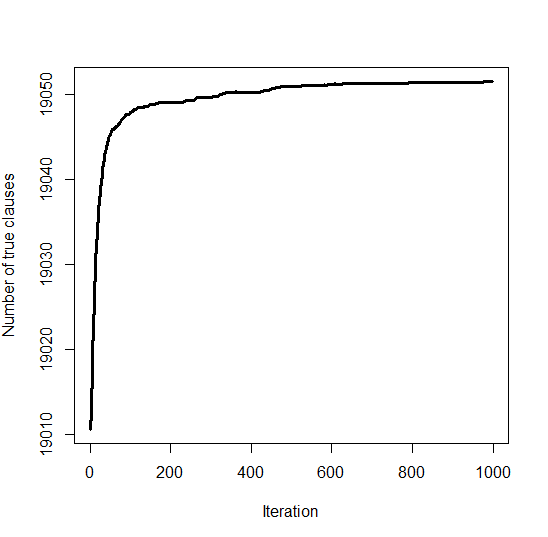
\includegraphics[width=\linewidth]{30-15.png}
  \caption{30-15}
\end{figure}
\begin{figure}[H]
  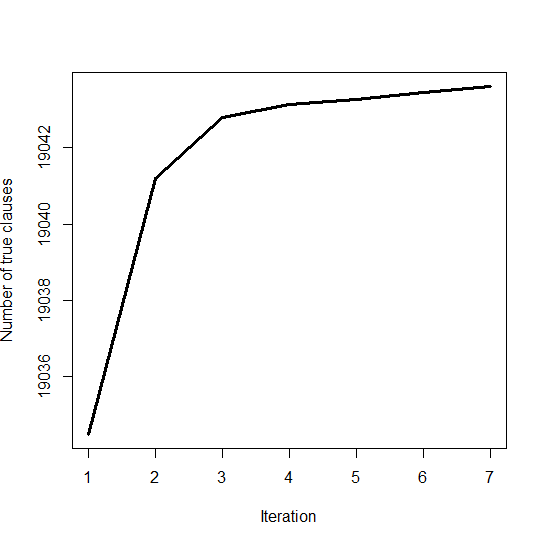
\includegraphics[width=\linewidth]{30-15-HC.png}
  \caption{30-15-HC}
\end{figure}
\begin{figure}[H]
  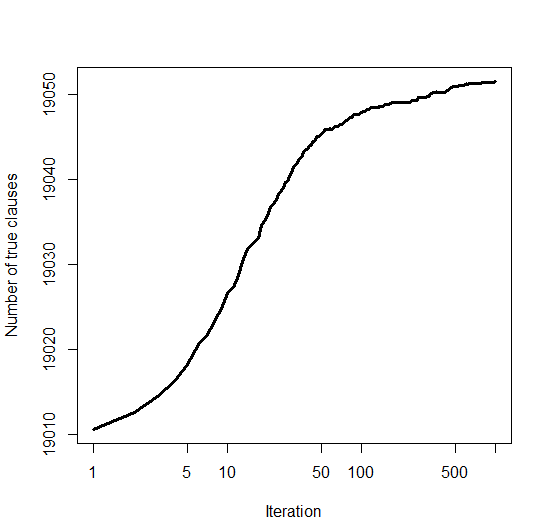
\includegraphics[width=\linewidth]{30-15-log.png}
  \caption{30-15-log}
\end{figure}
\begin{figure}[H]
  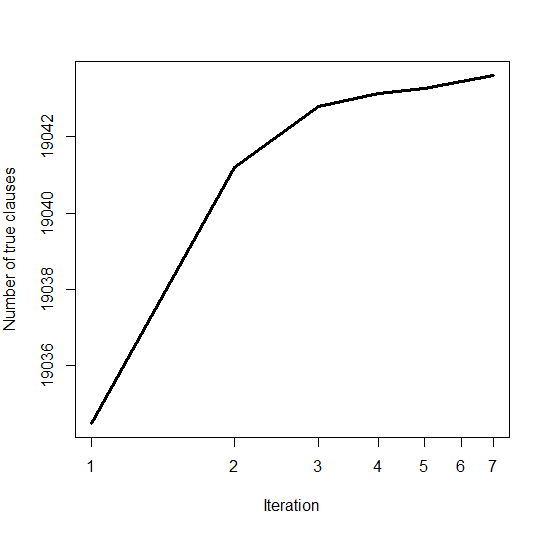
\includegraphics[width=\linewidth]{30-15-HC-log.png}
  \caption{30-15-HC-log}
\end{figure}

The first input had relatively good results on the GA, it found 18/30 runs the final answers. While the HC had 0 /30 final answers. The average for GA was at 19049,48 and for HC was 19045,04.



\subsection{35-17}
\begin{figure}[H]
  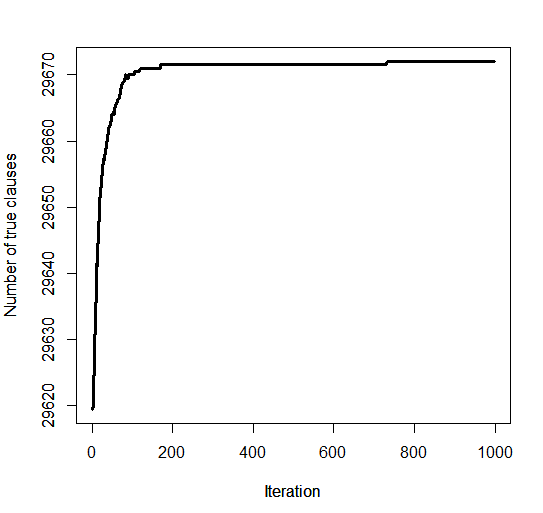
\includegraphics[width=\linewidth]{35-17.png}
  \caption{35-17}
\end{figure}
\begin{figure}[H]
  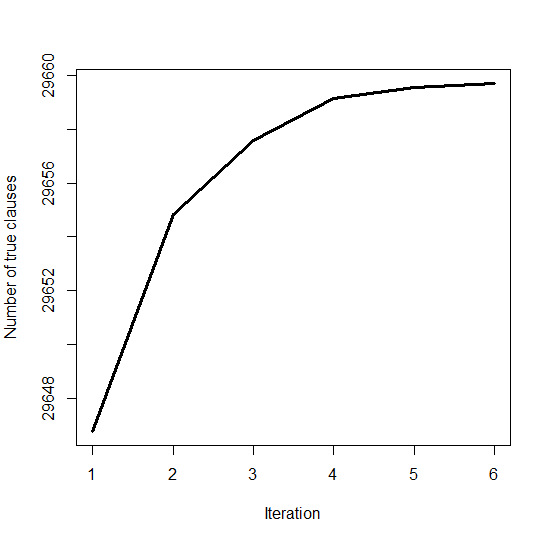
\includegraphics[width=\linewidth]{35-17-HC.png}
  \caption{35-17-HC}
\end{figure}
\begin{figure}[H]
  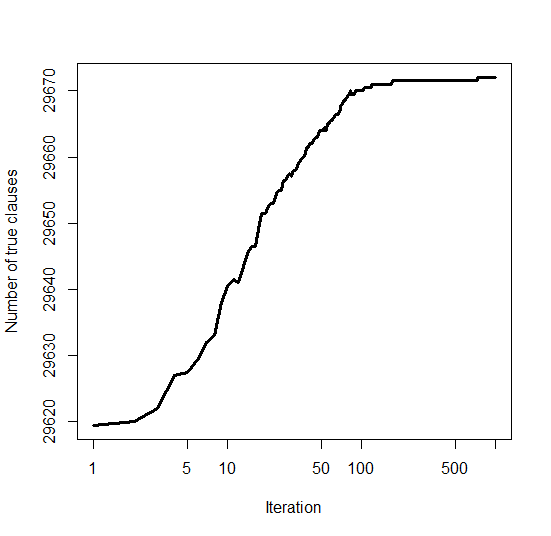
\includegraphics[width=\linewidth]{35-17-log.png}
  \caption{35-17-log}
\end{figure}
\begin{figure}[H]
  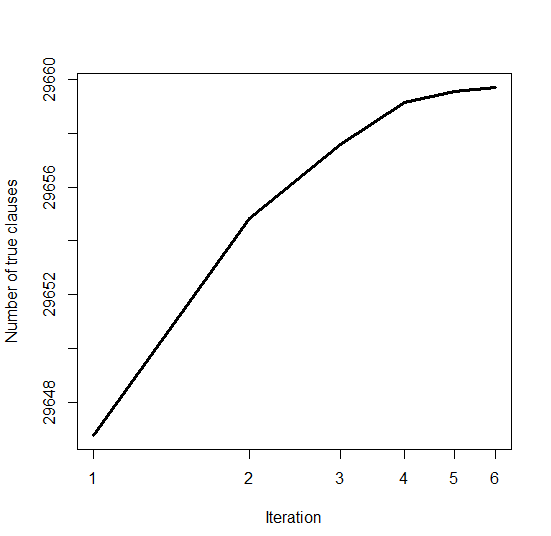
\includegraphics[width=\linewidth]{35-17-HC-log.png}
  \caption{35-17-HC-log}
\end{figure}
On the second input, GA found 5/30 assignments that could satisfy the given problem. The HC got again 0.
The average for GA was at 29665,32 and for HC was 29659,54.


\subsection{40-19}
\begin{figure}[H]
  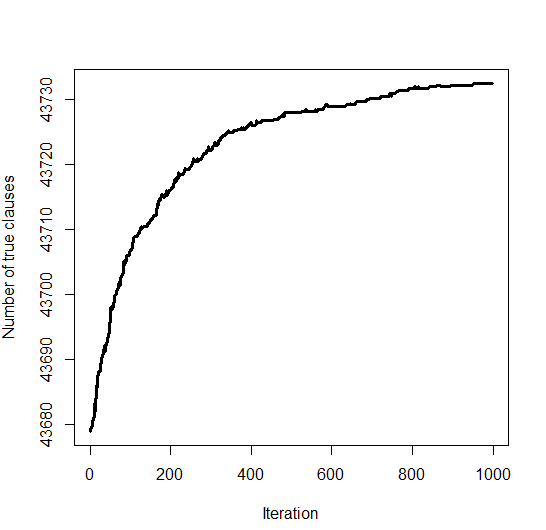
\includegraphics[width=\linewidth]{40-19.png}
  \caption{40-19}
\end{figure}
\begin{figure}[H]
  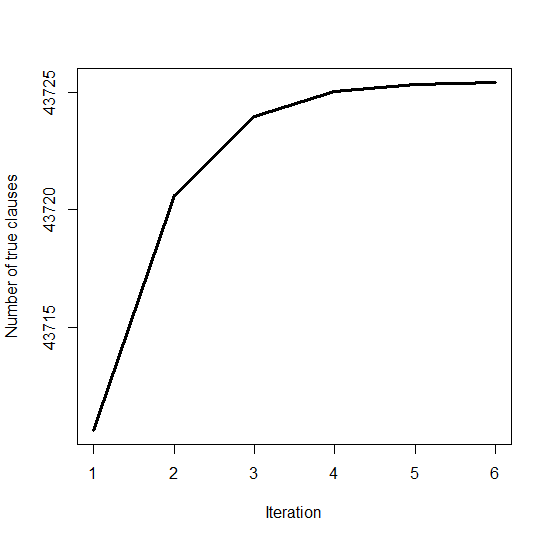
\includegraphics[width=\linewidth]{40-19-HC.png}
  \caption{40-19-HC}
\end{figure}
\begin{figure}[H]
  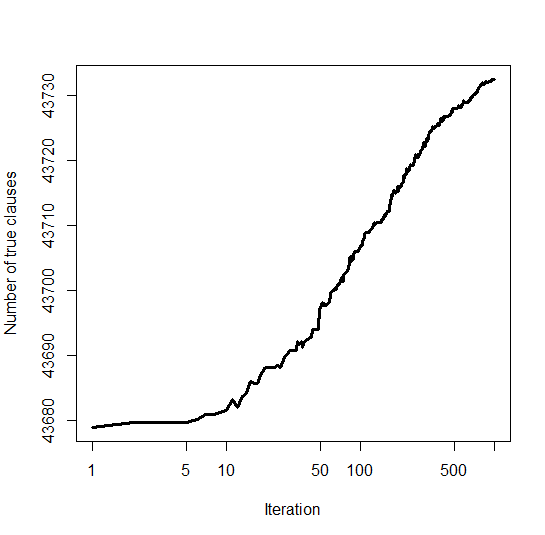
\includegraphics[width=\linewidth]{40-19-log.png}
  \caption{40-19-log}
\end{figure}
\begin{figure}[H]
  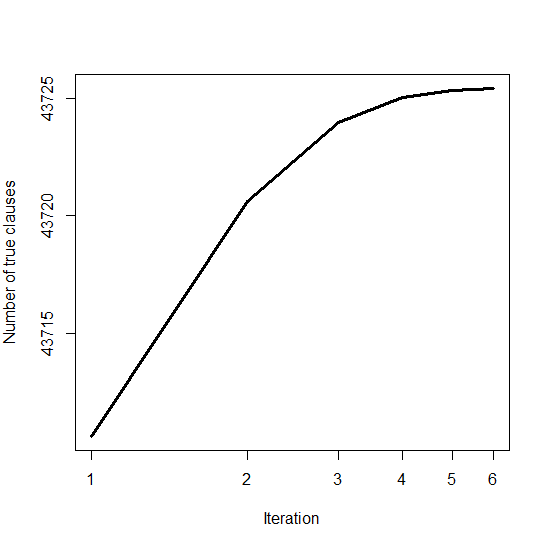
\includegraphics[width=\linewidth]{40-19-HC-log.png}
  \caption{40-19-HC-log}
\end{figure}
Average for GA was 43737.522 while for the HC it was 43725.32
This was the hardest input by far, the GA found the answer in only 2 out of 30 runs. It still an improvement from HC that got 0.



\section{Conclusion}

In all cases, the genetic algorithm was better overall, but not extraordinarily.
First improvement HC is a lot faster (in about 5/6 iterations), but it was always reaching a local maximum.
A possibility of GA are those that it can be tweeked and applied to a specific problem, gaining an advantage over other algorithms that apply generally. Another posibility is that a supervisor GA can be added to further advance the capabilities. 





%----------------------------------------------------------------------------------------
%	SECTION 5
%----------------------------------------------------------------------------------------


%
% ---- Bibliography ----\
%

\begin{thebibliography}{1}

\bibitem{ref1}
 Martin Davis and Hilary Putnam. A computing procedure for quantification theory. J. ACM, 7(3):201–215, July 1960.

\bibitem{input}
http://sites.nlsde.buaa.edu.cn/~kexu/benchmarks/benchmarks.htm

\end{thebibliography}  


\end{document}